\section*{Introduction}
\noindent This assignment is a practice to solve face recognition problem using different pattern recognition methods. In first two parts, \textit{Principal Component Analysis} (PCA) and \textit{Linear Discriminant Analysis} (LDA) are used to reduced the dimensionality of the data, followed by \textit{k-Nearest Neighbors} (KNN), first nearest neighbor in this assignment, to classify the faces. The last two parts are to use \textit{Support Vector Machine} (SVM) and \textit{Convolutional Neural Network} (CNN) to classify the faces.

\section*{Dataset}
\noindent The project will be conducted on the \textit{CMU PIE dataset2} and 10 selfie images. There are in total 68 different subjects plus one selfie. The training process is based on 70\% of 20 randomly selected subjects and 7 self-taking images while test is based on 30\% of the randomly selected subjects and 3 self-taking images. Due to the relatively small training and test size for self-taking images, the classification accuracy for self-taking images are quite low, yet the overall accuracy is satisfying enough with such simple methods.

\section*{PCA for Feature Extraction, Visualization and Classification}
\noindent The size of raw face image is 32$\times$32 pixels, resulting in a 1024 dimensional vector for each image. However, images may not be accurately classified because of the curse dimentionality with the classification method (KNN) we used. In this case, it is necessary to reduce the dimension of the data before passing to the classification model. PCA is a classic unsupervised dimension reduction method. 

The basic idea of PCA is to find a new sets of eigenvectors and eigenvalues to represent the data with minimal data loss. Then the new data is reconstructed based on the eignevectors.

\vspace{5mm}
\noindent \textbf{Steps:}\hfill \break
1. Compute the covariance matrix;\hfill \break
2. Perform eigenvalue decomposition;\hfill \break
3. Output PCs matrix.\hfill \break
\vspace{5mm}

Let $\{ \vec{x}_i \}$ be a set of $N$ column vectors of dimension $D$ ($D=1024$).
Define the covariance matrix ${\bf \rm S}_x$ of the dataset as
$$
	{\bf \rm S}_x = \frac{1}{N} \sum^N_{i=1} ( x_i - \bar{x} )( x_i - \bar{x} )^{T}
$$
where $\bar{x}$ is the mean of the dataset:
$$
	\bar{x} = \frac{1}{N} \sum^N_{i=1} x_i
$$

The $d$ largest principle components are the eigenvectors
$\vec{w}_i$ corresponding to the $d$ largest eigenvalues. The eigenvectors of {\bf S} can usually be found by using 
singular value decomposition. The $d$ eigenvectors can also be used to project the data into a
$d$ dimensional space.
Define
$$
{\bf \rm W} = [\vec{\mu}_1, \vec{\mu}_2, \dots, \vec{\mu}_d ]
$$
The projection of vector $\vec{x}$ is $\vec{y} = {\bf \rm W}^T \vec{x}$.
The corresponding scatter matrix ${\bf \rm S}_y$ of the
vectors $\{ \vec{y}_i \}$ is:
$$
{\bf \rm S}_y = {\bf \rm W}^T {\bf \rm S}_x {\bf \rm W}
$$

When the image data's dimension is reduced to 2, it can be visualized in a 2D plane.
When the image data's dimension is reduced to 3, it can be visualized in a 3D space.

By choosing the first 3 eigenvectors, the first 3 eigenfaces can be plotted as follows.

\subsection*{Implementation in Python}
\begin{lstlisting}
functions in  Python ...
## function for calculating basic characteristics
basicchar <- function(x){
  v1 <- c(length(x), round(mean(x),2), round(sd(x),2))
  return(v1)
}
# calculating basic characteristics of women and of men
women <- basicchar(data$skull.height[data$sex == 'F'])
men <- basicchar(data$skull.height[data$sex == 'M'])
tab <- rbind(women, men)
# plotting boxplots
boxplot(data$skull.height[data$sex == 'F'], 
        data$skull.height[data$sex == 'M'],
        col = "steelblue", 
        xlab = "",
        ylab = "Skull Height (mm)",
        xaxt = "n", 
        boxwex = 0.5)
axis(1, at = 1:2, labels = c("women","men"))
# adding averages
points(tab[,2], col = "red", pch = 16)
\end{lstlisting}

You will submit your complete code in an \textsf{.R} file or an \textsf{.Rnw} file according to the instructions for the assignments. Only required functions or parts of code crucial to the exercise will be inserted here.
\bigskip
\subsection*{Results and interpretation}
\noindent Text. Results in table or graphic form. Commentaries and interpretation of the results.

 Interpretation. Text. Commentary relating to tables and figures. What can we infere about the differences in skull height between men and women from the values in the table? How can we know from the figure, whether our data come from a normal distribution?

\begin{table}[ht]
\footnotesize
\centering

\begin{tabular}{r||rrr}
 Gender & Number of individuals & Average skull height (mm) & Standard deviation \\ 
 \hline \hline
Women & 20 & 127.70 & 6.86 \\ 
Men & 40 & 135.54 & 5.20 \\ 
\end{tabular}
\caption{Basic characteristics of skull height of women and of men}
\end{table}


\begin{figure}[ht]
\centering
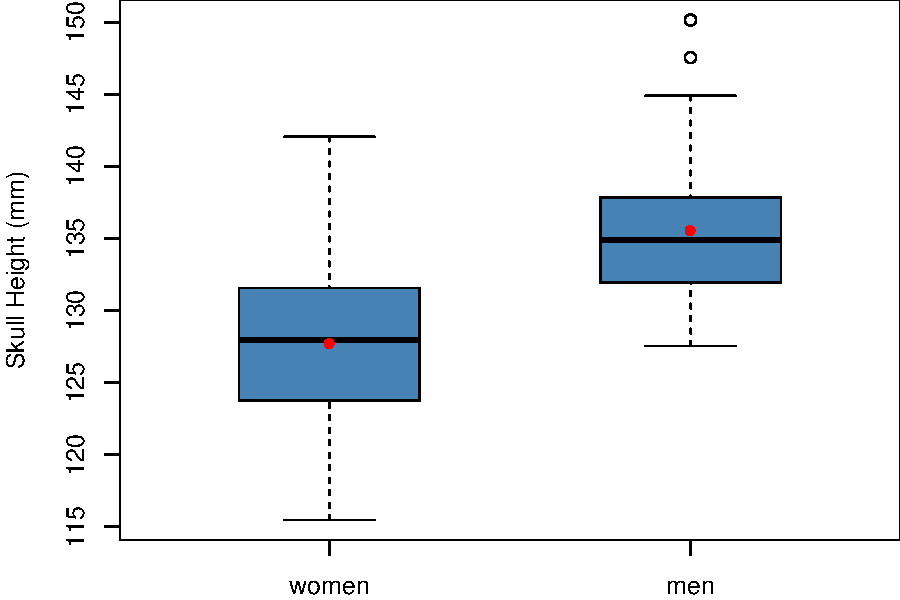
\includegraphics[angle=0,width=0.45\textwidth]{boxplot-example.pdf}
\caption{Boxplots of skull height of women and of men}
\end{figure}

\newpage

\section*{2. LDA for Feature Extraction and Classification}
\noindent Text. Commentary on the approach to solving the exercise, theoretical derivation if the assignment asks for it.

Text. Paragraphs are separated by an empty line. 

\subsection*{Implementation in R}
\begin{lstlisting}
functions in  R ...
## function for calculating basic characteristics
basicchar <- function(x){
  v1 <- c(length(x), round(mean(x),2), round(sd(x),2))
  return(v1)
}
# calculating basic characteristics of women and of men
women <- basicchar(data$skull.height[data$sex == 'F'])
men <- basicchar(data$skull.height[data$sex == 'M'])
tab <- rbind(women, men)
# plotting boxplots
boxplot(data$skull.height[data$sex == 'F'], 
        data$skull.height[data$sex == 'M'],
        col = "steelblue", 
        xlab = "",
        ylab = "Skull Height (mm)",
        xaxt = "n", 
        boxwex = 0.5)
axis(1, at = 1:2, labels = c("women","men"))
# adding averages
points(tab[,2], col = "red", pch = 16)
\end{lstlisting}

You will submit your complete code in an \textsf{.R} file or an \textsf{.Rnw} file according to the instructions for the assignments. Only required functions or parts of code crucial to the exercise will be inserted here.
\bigskip
\subsection*{Results and interpretation}
\noindent Text. Results in table or graphic form. Commentaries and interpretation of the results.

 Interpretation. Text. Commentary relating to tables and figures. What can we infere about the differences in skull height between men and women from the values in the table? How can we know from the figure, whether our data come from a normal distribution?

\begin{table}[ht]
\footnotesize
\centering

\begin{tabular}{r||rrr}
 Gender & Number of individuals & Average skull height (mm) & Standard deviation \\ 
 \hline \hline
Women & 20 & 127.70 & 6.86 \\ 
Men & 40 & 135.54 & 5.20 \\ 
\end{tabular}
\caption{Basic characteristics of skull height of women and of men}
\end{table}


\begin{figure}[ht]
\centering
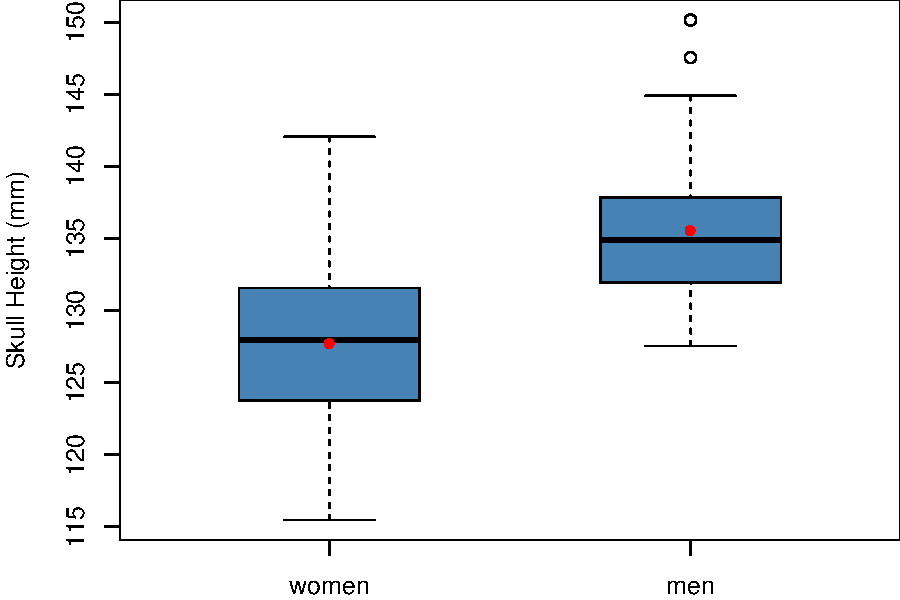
\includegraphics[angle=0,width=0.45\textwidth]{boxplot-example.pdf}
\caption{Boxplots of skull height of women and of men}
\end{figure}

\section*{3. SVM for Classification}
\noindent Text. Commentary on the approach to solving the exercise, theoretical derivation if the assignment asks for it.

Text. Paragraphs are separated by an empty line. 

\subsection*{Implementation in R}
\begin{lstlisting}
functions in  R ...
## function for calculating basic characteristics
basicchar <- function(x){
  v1 <- c(length(x), round(mean(x),2), round(sd(x),2))
  return(v1)
}
# calculating basic characteristics of women and of men
women <- basicchar(data$skull.height[data$sex == 'F'])
men <- basicchar(data$skull.height[data$sex == 'M'])
tab <- rbind(women, men)
# plotting boxplots
boxplot(data$skull.height[data$sex == 'F'], 
        data$skull.height[data$sex == 'M'],
        col = "steelblue", 
        xlab = "",
        ylab = "Skull Height (mm)",
        xaxt = "n", 
        boxwex = 0.5)
axis(1, at = 1:2, labels = c("women","men"))
# adding averages
points(tab[,2], col = "red", pch = 16)
\end{lstlisting}

You will submit your complete code in an \textsf{.R} file or an \textsf{.Rnw} file according to the instructions for the assignments. Only required functions or parts of code crucial to the exercise will be inserted here.
\bigskip
\subsection*{Results and interpretation}
\noindent Text. Results in table or graphic form. Commentaries and interpretation of the results.

 Interpretation. Text. Commentary relating to tables and figures. What can we infere about the differences in skull height between men and women from the values in the table? How can we know from the figure, whether our data come from a normal distribution?

\begin{table}[ht]
\footnotesize
\centering

\begin{tabular}{r||rrr}
 Gender & Number of individuals & Average skull height (mm) & Standard deviation \\ 
 \hline \hline
Women & 20 & 127.70 & 6.86 \\ 
Men & 40 & 135.54 & 5.20 \\ 
\end{tabular}
\caption{Basic characteristics of skull height of women and of men}
\end{table}


\begin{figure}[ht]
\centering
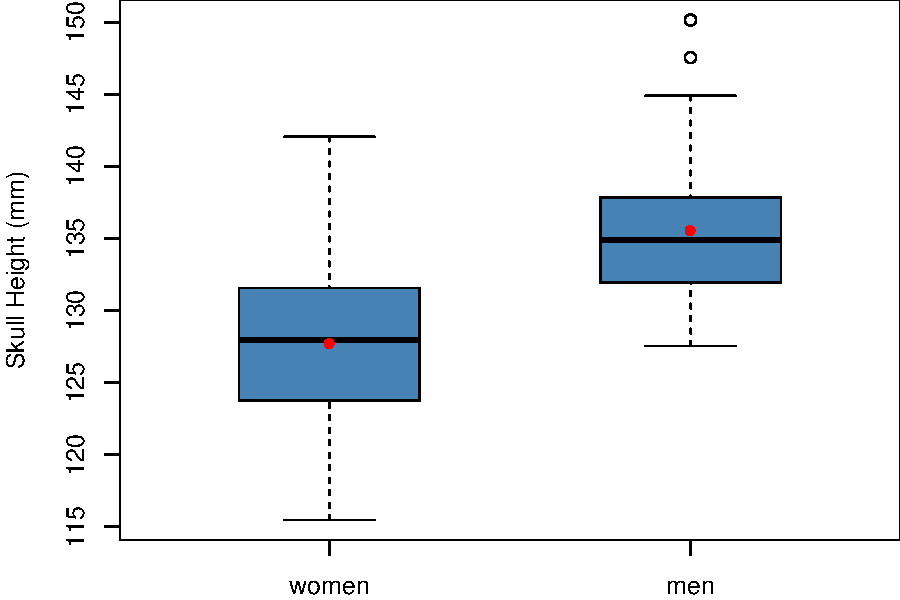
\includegraphics[angle=0,width=0.45\textwidth]{boxplot-example.pdf}
\caption{Boxplots of skull height of women and of men}
\end{figure}

\newpage

\section*{4. Neural Networks}
\noindent Text. Commentary on the approach to solving the exercise, theoretical derivation if the assignment asks for it.

Text. Paragraphs are separated by an empty line. 

\subsection*{Implementation in R}
\begin{lstlisting}
functions in  R ...
## function for calculating basic characteristics
basicchar <- function(x){
  v1 <- c(length(x), round(mean(x),2), round(sd(x),2))
  return(v1)
}
# calculating basic characteristics of women and of men
women <- basicchar(data$skull.height[data$sex == 'F'])
men <- basicchar(data$skull.height[data$sex == 'M'])
tab <- rbind(women, men)
# plotting boxplots
boxplot(data$skull.height[data$sex == 'F'], 
        data$skull.height[data$sex == 'M'],
        col = "steelblue", 
        xlab = "",
        ylab = "Skull Height (mm)",
        xaxt = "n", 
        boxwex = 0.5)
axis(1, at = 1:2, labels = c("women","men"))
# adding averages
points(tab[,2], col = "red", pch = 16)
\end{lstlisting}

You will submit your complete code in an \textsf{.R} file or an \textsf{.Rnw} file according to the instructions for the assignments. Only required functions or parts of code crucial to the exercise will be inserted here.
\bigskip
\subsection*{Results and interpretation}
\noindent Text. Results in table or graphic form. Commentaries and interpretation of the results.

 Interpretation. Text. Commentary relating to tables and figures. What can we infere about the differences in skull height between men and women from the values in the table? How can we know from the figure, whether our data come from a normal distribution?

\begin{table}[ht]
\footnotesize
\centering

\begin{tabular}{r||rrr}
 Gender & Number of individuals & Average skull height (mm) & Standard deviation \\ 
 \hline \hline
Women & 20 & 127.70 & 6.86 \\ 
Men & 40 & 135.54 & 5.20 \\ 
\end{tabular}
\caption{Basic characteristics of skull height of women and of men}
\end{table}


\begin{figure}[ht]
\centering
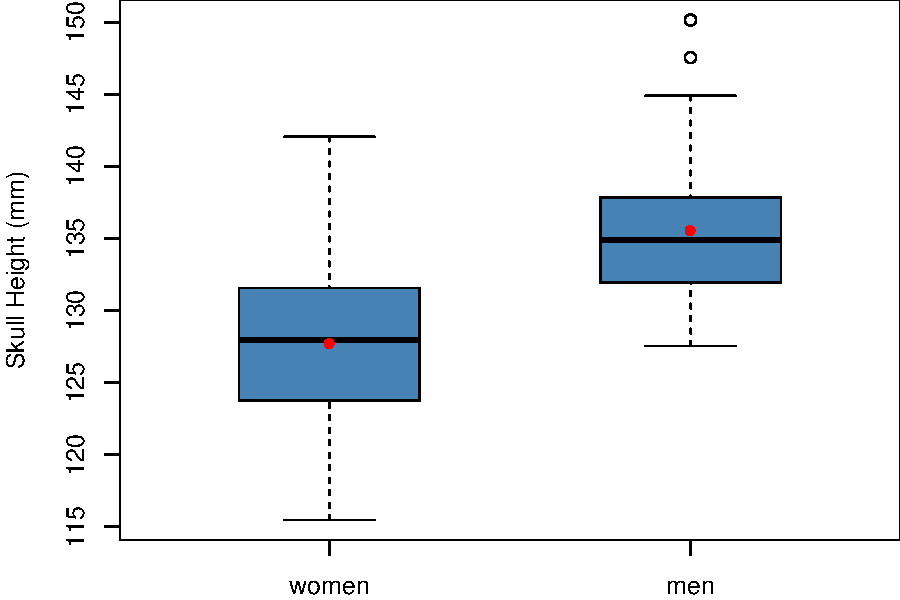
\includegraphics[angle=0,width=0.45\textwidth]{boxplot-example.pdf}
\caption{Boxplots of skull height of women and of men}
\end{figure}